\documentclass[11pt]{beamer}
\usetheme{metropolis}
\usepackage[utf8]{inputenc}
\usepackage[english]{babel}
\usepackage[T1]{fontenc}
\usepackage{amsmath}
\usepackage{amsfonts}
\usepackage{amssymb}
\usepackage{bm}
\usepackage{tikz}
\usetikzlibrary{tikzmark,decorations.pathreplacing,calligraphy}
\usepackage{subfig}
\usepackage{pgfplots}
\pgfplotsset{compat=newest}
\usepackage{multimedia}
%\usepackage{booktabs}
\newcommand{\Ex}{\mathbb{E}}
\newcommand{\Var}{\mathbb{V}\mathrm{ar}}
\newcommand{\Prob}{\mathbb{P}}
\DeclareMathOperator*{\argmin}{arg\,min}
\DeclareMathOperator*{\argmax}{arg\,max}
\newcommand{\Cov}{\textsf{Cov}}
\newcommand{\tra}{\mathrm{tr}}
\newcommand{\yobs}{\bm{y}^{\mathrm{obs}}}
\newcommand{\kest}{\hat{\bm{k}}}
\usetikzlibrary{positioning}
\DeclareMathOperator*{\KL}{\textsf{KL}}
\graphicspath{{../Figures/}}

\definecolor{blkcol}{HTML}{E1E1EA}
\definecolor{blkcol2}{RGB}{209, 224, 224}

% \definecolor{BlueTOL}{HTML}{222255}
% \definecolor{BrownTOL}{HTML}{666633}
% \definecolor{GreenTOL}{HTML}{225522}
% \setbeamercolor{normal text}{fg=BlueTOL,bg=white}
% \setbeamercolor{alerted text}{fg=BrownTOL}
% \setbeamercolor{example text}{fg=GreenTOL}
\setbeamercolor{block title}{bg = blkcol}
\setbeamercolor{block body}{bg = blkcol!50}


\title{Parameter control in the presence of uncertainties}
\author{{\large Victor Trappler } \\ Supervisors: Élise Arnaud, Laurent Debreu, Arthur Vidard}
\institute{AIRSEA Research team (Inria)-- Laboratoire Jean Kuntzmann \\
 \begin{center}
\includegraphics[scale=0.20]{INRIA_SCIENTIFIQUE_UK_CMJN}
\includegraphics[scale=0.20]{ljk}
\end{center}
}

\date{\today}
\setcounter{tocdepth}{1}


\begin{document}
\frame{
  \maketitle
}

% \section{Introduction}
\frame{
\frametitle{Friction de fond}
\begin{itemize}
\item Friction du fond a une influence sur la circulation de l'eau en surgace
\item Dépend de la taille caractéristique des aspérités
\item Phénomène sous-maille
\end{itemize}
\begin{center}
\input{../Figures/hauteureau.tikz}
\end{center}

}
% \frame{
% %   \frametitle{Principles of Computer experiments}
% %   \scalebox{0.7}{\input{../Figures/schema_bloc}}
% % }

% \frame{
% \frametitle{Outline}
% \tableofcontents
% }
% \section{Problème classique sans incertitudes}
\frame[t]{
\frametitle{Modèle numérique: Shallow Water Equations}
% \begin{itemize}
% 	\item[Input] 
% 	\begin{itemize}
% 		\item $\bm{k}$: Bottom friction (spatially distributed)
% 		\item $\bm{u}$: Environmental variables (fixed and known)
% 	\end{itemize}
% 	\item[Output] \begin{itemize}
% 	\item $W(\bm{k}) = \{W_i^n(\bm{k})\}_{i,n}$, where $W_i^n(\bm{k}) = [h_i^n(\bm{k}) \quad q_i^n(\bm{k})]^T$\\ for $0 \leq i \leq N_x$ and $0 \leq n \leq N_t$
% 	\end{itemize}
% \end{itemize}
\vfill
% \only<1>{\tikzstyle{block} = [rectangle, draw, fill=blue!20, 
     text centered, minimum width=1cm]

\tikzstyle{block2} = [rectangle, draw, fill=green!20, 
     text centered, rounded corners, minimum width=1cm]

\tikzstyle{LHS}=[rectangle, draw, text centered]

\begin{tikzpicture}[node distance=3cm]

\node [align = center] at (0,0) (input) {Control variable \\$K \in \mathcal{K}$};
%\node [align = center] at (4,1.5) (envir) {Environmental variables \\$\bm{u} \in \mathcal{U}$ fixed};
\node [align = center] at (4,1.5) (envir) {Environmental variables \\$\bm{x}_e \in \mathbb{X}$ fixed};

\node[block] at (4,0)(code){Direct Simulation};

\node[align = center] at (8,0) (output) {$W(K)$}; %\\ $\Rightarrow j(K)$};

\draw[->] (input) -- (code);
\draw[->] (envir) -- (code);
\draw[->] (code) -- (output);

\end{tikzpicture}}
\only<1>{\usetikzlibrary{positioning}
% \tikzstyle{block} = [rectangle, draw, fill=blue!30, 
%     text centered, minimum width=3em] 
 \tikzstyle{block} = [rectangle, draw, fill=blkcol, 
      text centered, minimum width=3em]

\tikzstyle{block2} = [rectangle, draw, fill=blkcol2, 
     text centered, rounded corners, minimum width=3em]

% \tikzstyle{block2} = [rectangle, draw, fill=blkcol2, 
%      text centered, rounded corners, minimum width=3em]

\tikzstyle{LHS}=[rectangle, draw, text centered]

\begin{tikzpicture}

%\node [align = center] at (0,0) (input) {Control variable \\$\mathbf{k} \in \Kspace$};
\node [align = center] at (0,0) (input) {Control variable \\$\theta \in \Kspace$};
\node[block] at (4,0) (code){Direct Simulation};
%\node [align = center, above =of  code ] (envir) {Environmental variables \\$\mathbf{u} \in \Uspace$ fixed};
\node [align = center] at (4,1.5) (envir) {Environmental variables \\$\uu \in \Uspace$ fixed};




\node[align = center] at (8,0) (output) {$\mathcal{M}(\theta,\uu)$};
\node [align = center] at (8,-1) (obs) {$\yobs$};
\node[block] at (4,-1) (inv) {Inverse Problem};

\draw[->] (input) -- (code);
\draw[->] (envir) -- (code);
\draw[->] (code) -- (output);

 % \node [align = center] at (0,0) (input) {$Y = \mathbb{H}M(K_{\mathrm{ref}})$};
 % \node [align = center] at (4,1.5) (envir) {Environmental variables \\$X_e$ r.v.};

 % \node[block] at (4,0)(code){"Inverse Problem"};

% \node[align = center] at (8,0) (output) {$K$};

\draw[->] (input) -- (code);
% \draw[->] (envir) -- (code);
\draw[->] (code) -- (output);
\draw[->] (output) -- (obs) ;
\draw[->] (inv) -|(input) ;
\draw[->] (obs) -- (inv);
\end{tikzpicture}}

\textbf{Expériences jumelles}: On choisit $\bm{k}_{\mathrm{ref}}$\\
On a donc  $\yobs = M(\bm{k}_{\mathrm{ref}})$
\begin{itemize}
\item  Fonction coût: $J(\bm{k}) = \frac12 \|M(\bm{k}) - \bm{y}^{\mathrm{obs}} \|^2 + \text{Régul. eventuelle}$
\item  Estimateur : $\kest = \argmin_{\bm{k} \in \mathcal{K}}J(\bm{k})$
\end{itemize}
}
% \frame{
% \frametitle{Data assimilation framework: Twin experiments}

%\begin{itemize}
%\item<2-> Gradient-free: Simulated annealing, Nelder-mead,\dots
%$\rightarrow$ High number of runs, \alert<2>{very expensive}
%
%\item<3-> Gradient-based: gradient-descent, (quasi-) Newton method
%$\rightarrow$ Less number of runs, but \alert<3>{need the adjoint code}
%\end{itemize}
% }
% \section{Estimation sous incertitudes}
\frame[t]{
\frametitle{Incertitudes dans un code déterministe}
$\bm{U}$ est maintenant une variable aléatoire (densité $\pi(\bm{u})$) \\ $\yobs$ a été générée avec $\bm{u}_{\mathrm{ref}}$, échantillon de $\bm{U}$
\vfill
% \only<1>{\usetikzlibrary{positioning}
% \tikzstyle{block} = [rectangle, draw, fill=blue!30, 
%     text centered, minimum width=3em] 
 \tikzstyle{block} = [rectangle, draw, fill=blkcol, 
      text centered, minimum width=3em]

\tikzstyle{block2} = [rectangle, draw, fill=blkcol2, 
     text centered, rounded corners, minimum width=3em]

% \tikzstyle{block2} = [rectangle, draw, fill=blkcol2, 
%      text centered, rounded corners, minimum width=3em]

\tikzstyle{LHS}=[rectangle, draw, text centered]

\begin{tikzpicture}

%\node [align = center] at (0,0) (input) {Control variable \\$\mathbf{k} \in \Kspace$};
\node [align = center] at (0,0) (input) {Control variable \\$\theta \in \Kspace$};
\node[block] at (4,0) (code){Direct Simulation};
%\node [align = center, above =of  code ] (envir) {Environmental variables \\$\mathbf{u} \in \Uspace$ fixed};
\node [align = center] at (4,1.5) (envir) {Environmental variables \\$\uu \in \Uspace$ fixed};




\node[align = center] at (8,0) (output) {$\mathcal{M}(\theta,\uu)$};
\node [align = center] at (8,-1) (obs) {$\yobs$};
\node[block] at (4,-1) (inv) {Inverse Problem};

\draw[->] (input) -- (code);
\draw[->] (envir) -- (code);
\draw[->] (code) -- (output);

 % \node [align = center] at (0,0) (input) {$Y = \mathbb{H}M(K_{\mathrm{ref}})$};
 % \node [align = center] at (4,1.5) (envir) {Environmental variables \\$X_e$ r.v.};

 % \node[block] at (4,0)(code){"Inverse Problem"};

% \node[align = center] at (8,0) (output) {$K$};

\draw[->] (input) -- (code);
% \draw[->] (envir) -- (code);
\draw[->] (code) -- (output);
\draw[->] (output) -- (obs) ;
\draw[->] (inv) -|(input) ;
\draw[->] (obs) -- (inv);
\end{tikzpicture}}
\only<1>{\input{../Figures/comp_code_unc_inv_noalert.pgf}}

\begin{itemize}
\item $M(\bm{k}) \quad \text{devient} \quad M(\bm{k},\bm{u})$ ($\bm{u}$ est une entrée du modèle)
\item Fonction coût: $J(\bm{k},\bm{u}) =  \frac12\|M(\bm{k},\bm{u}) - \yobs\|^2$ + \text{Régul}
\end{itemize}
}
\begin{frame}
  \frametitle{Estimateur robuste ?}
  On veut pouvoir trouver une valeur $\kest$, tel que $M(\kest,\bm{U})$ soit relativement semblable à $\yobs$

  

  Idéalement, $M(\kest,\cdot)$
  \begin{itemize}
  \item reste assez performant pour fournir des prédictions acceptables
  \item ne varie pas trop avec $\bm{U}$
  \end{itemize}
\end{frame}
\frame{
\frametitle{Approche variationnelle ou Bayésienne ?}
\begin{itemize}
\item<1-> \textbf{Variationnelle}: Variable aléatoire indexée par $\bm{k}$: $\bm{k} \mapsto J(\bm{k},\bm{U})$, \\ Extrema des moments ? $\Ex[J(\bm{K},\bm{U})|\bm{K} = \bm{k}] \dots$
\item<1-> \textbf{Bayésienne}:  $e^{-J(\bm{k},\bm{u})} \propto p(\yobs|\bm{k},\bm{u})$= Vraisemblance  \\ Inférence bayésienne, marginalisation, Estimation bayésienne
\end{itemize}
\onslide<1-> Mais
\begin{itemize}
\item Estimer efficacement moments ?
\item Quelle connaissance de $\bm{U}$ ?
\item Gérer le coût de calcul du modèle
\end{itemize}
}
%\frame{
%\frametitle{Issues raised}
%%Random variable : $J(\bm{X}_e,K)$
%\begin{tabular}{ll}
%Influence of $\bm{X}_e$ ? & \onslide<2->{ $\longrightarrow$ Sensitivity analysis}\\
%Computational cost ? & \onslide<2->{ $\longrightarrow$ Use of surrogate}
%\end{tabular}
%}


% \section{Estimateurs ``robustes''}

% \subsection{Concepts of robustness}
% \frame{
% 	\frametitle{An illustration}
% 	$(\bm{u},\bm{k}) \mapsto f(\bm{u},\bm{k}) = \tilde{f}(\bm{u}+\bm{k})$ \\ $\bm{U} \sim \mathcal{N}(0,s^2)$ truncated on $[{-3};3]$. Plot of $f(0,\cdot) = \tilde{f}(\cdot)$ \vfill
% 	\begin{figure}[!h]
% 	\centering
% 	\includegraphics[scale = 0.5]{../Figures/mean_worstcase_robustness1}
% 	\end{figure}
% }
% \frame{
% 	\frametitle{An illustration}
% 	$(\bm{u},\bm{k}) \mapsto f(\bm{u},\bm{k}) = \tilde{f}(\bm{u}+\bm{k})$ \\ $\bm{U} \sim \mathcal{N}(0,s^2)$ truncated on $[{-3};3]$. {\color{red}	Plot of $\max_{\bm{u}} \{f(\bm{u},\cdot)\}$} \vfill
% 	\begin{figure}[!h]
% 	\centering
% 	\includegraphics[scale = 0.5]{../Figures/mean_worstcase_robustness2}
% 	\end{figure}
% }
% \frame{
% 	\frametitle{An illustration}
% 	$(\bm{u},\bm{k}) \mapsto f(\bm{u},\bm{k}) = \tilde{f}(\bm{u}+\bm{k})$ \\ $\bm{U} \sim \mathcal{N}(0,s^2)$ truncated on $[{-3};3]$. {\color{green} Plot of $\Ex_{\bm{u}}[f(\bm{u},\cdot)]$} \vfill
% 	\begin{figure}[!h]
% 	\centering
% 	\includegraphics[scale = 0.5]{../Figures/mean_worstcase_robustness3}
% 	\end{figure}
% }
\frame{
  \frametitle{Différents critères}
  % \textbf{Non-exhaustive list of ``Robust'' Objectives }
\begin{itemize}
\item Optimum global: $ \min_{(\bm{k},\bm{u})} J(\bm{k},\bm{u})$ $ \longrightarrow $ EGO \tikzmark{start1} 
\item Pire des cas: $ \min_{\bm{k}} \max_{\bm{u}} J(\bm{k},\bm{u})$ $ \longrightarrow $ Explorative EGO \tikzmark{end1} 
\item M-robustesse: $\min_{\bm{k}} \Ex\left[J(\bm{k},\bm{U})\right] \longrightarrow $ iterated LHS \tikzmark{start2}
\item V-robustesse: $\min_{\bm{k}} \Var\left[J(\bm{k},\bm{U})\right] \longrightarrow $ gradient-descent with PCE
\item $\rho$-robustesse: $\min \rho(J(\bm{k},\bm{U}))$ $\longrightarrow$ gradient-descent with PCE
\item Multiobjectifs: estimer le front de Pareto $\longrightarrow$ 1L/2L kriging \tikzmark{end2}
\item Minimiser probabilité de défaillance: $\min_{\bm{k}} \Prob\left[J(\bm{k},\bm{U}) > T \right]$ \tikzmark{start3}
\item $\Prob\left[J(\bm{k},\bm{U}) \leq \min_{\tilde{\bm{k}}} J(\tilde{\bm{k}},\bm{U}) \right] = \Prob\left[\bm{k} = \argmin_{\tilde{\bm{k}}} J(\tilde{\bm{k}},\bm{U}) \right]$ \\
  $\rightarrow$ Distribution et mode de $\argmin_{\tilde{\bm{k}}} J(\tilde{\bm{k}},\bm{U})$: \alert{MPE}
\item Relaxation de la contrainte: $R_\alpha(\bm{k}) = \Prob\left[J(\bm{k},\bm{U}) \leq \alpha\min_{\tilde{\bm{k}}} J(\tilde{\bm{k}},\bm{U}) \right]$ \tikzmark{end3} 
\end{itemize}

\begin{tikzpicture}[remember picture,overlay]
  \draw[decorate,decoration={calligraphic brace}]
  ([yshift=10pt,xshift=10pt]{{pic cs:end1}|-{pic cs:start1}}) --
  node[xshift=5pt,anchor=west] {$\pi(\bm{u})$ ?}
  ([xshift=10pt]{pic cs:end1})
  ;
  \draw[decorate,decoration={calligraphic brace}]
  ([yshift=10pt,xshift=10pt]{{pic cs:end2}|-{pic cs:start2}}) --
  node[xshift=1pt,anchor=west] {$\substack{\Ex,\\\Var}$}
  ([xshift=10pt]{pic cs:end2})
  ;
  \draw[decorate,decoration={calligraphic brace}]
  ([yshift=10pt,xshift=85pt]{{pic cs:end3}|-{pic cs:start3}}) --
  node[xshift=1pt,anchor=west] {$\substack{\text{Random}\\\text{sets}}$}
  ([xshift=85pt]{pic cs:end3})
  ;
  
\end{tikzpicture}
}

\frame{
  \frametitle{Illustration en 2D: $\mathcal{K}\times\mathcal{U} = [0;5]^2$}
  \includegraphics[width = \textwidth]{../Figures/surface_transp_horiz.pdf}
}

\begin{frame}
  \frametitle{Illustration en 2D: relaxation de la contrainte avec $\alpha$}
  \includegraphics[width = \textwidth]{../Figures/alpha_relax}
\end{frame}

\frame{
  \frametitle{MPE et cluster, $\bm{u}_{\mathrm{ref}}$ centré}
  \begin{center}
    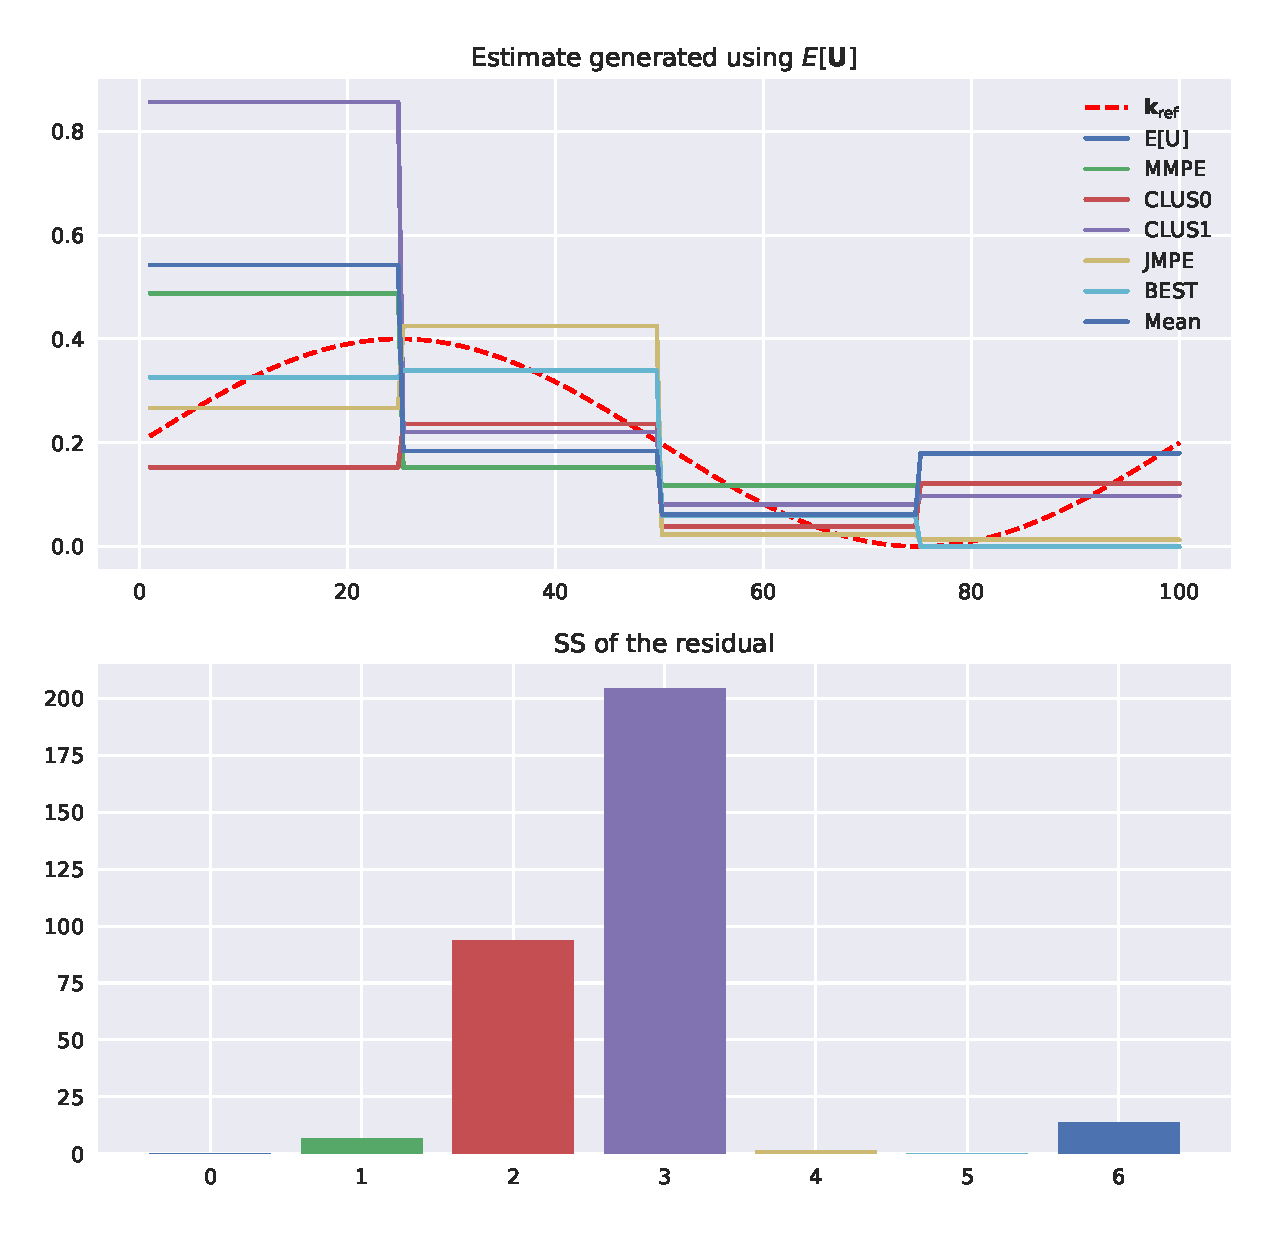
\includegraphics[width = \textheight]{../Figures/estimate_centered.eps}
    \end{center}
}

\frame{
  \frametitle{MPE et cluster,  $\bm{u}_{\mathrm{ref}}$ décalé}
  \begin{center}
    \includegraphics[width = \textheight]{../Figures/estimate_Am_Pm.eps}
  \end{center}

}

% \subsection{Formalisme bayésien}
\frame{
  \frametitle{Théorème de Bayes}
 On définit la distribution a priori de $\bm{K} \sim \pi(\bm{k})$.
  
 Distribution jointe de $(\bm{K},\bm{U})$ ayant observé $\yobs$:  $p(\bm{k},\bm{u}|\yobs)$ ? 
\begin{block}{Théorème de Bayes}
\begin{align*}
p(\bm{k},\bm{u} | \yobs) &\propto p(\yobs| \bm{k},\bm{u})\pi(\bm{k},\bm{u}) \\
					& \propto \alert{L(\bm{k},\bm{u}; \yobs)} \pi(\bm{k})\pi(\bm{u})
\end{align*}
\end{block}
Lien avec $J$ ?: Erreur quadratique $\leftrightarrow$ Erreur gaussienne
\begin{align*}
  L(\bm{k},\bm{u}; \yobs) &\propto \exp\left[- \tfrac{1}{2}\|M(\bm{k},\bm{u}) - \yobs \|^2_{\bm{\Sigma}^{-1}} \right] = \exp\left[-J(\bm{k},\bm{u})\right]
\end{align*}
}
\frame{
  \frametitle{Critères robustes Bayésiens}
% \newline
  % \begin{block}{Bayes' theorem}
  %   $p(\bm{k},\bm{u}|\yobs) \propto L(\bm{k},\bm{u}; \yobs) \pi(\bm{k})\pi(\bm{u})\propto \alert{p(\bm{k}|\yobs,\bm{u})}\pi(\bm{u})$
  %   \end{block}
    \begin{align*}
      \text{ML :}   & \quad\argmax_{(\bm{k},\bm{u})} L(\bm{k},\bm{u}; \yobs) \\
      \text{MAP :}  & \quad \argmax_{(\bm{k},\bm{u})} p(\bm{k},\bm{u}| \yobs)= L(\bm{k},\bm{u}; \yobs)\pi(\bm{k})\pi(\bm{u})\\
      \alert<1>{\text{MMAP :}} & \quad \argmax_{\bm{k}} p(\bm{k}|\yobs) = \int_{\mathcal{U}} p(\bm{k},\bm{u}| \yobs) \,\mathrm{d}\bm{u} \\
      \alert<1>{\text{Min variance :}} & \quad \argmin_{\bm{k}} \Var_{U}\left[p(\bm{k}| \yobs, \bm{U})\right] \\
      \alert<1>{\text{Pire des cas:}} & \quad \argmax_{\bm{k}} \{\min_{\bm{u}} p(\bm{k}|\yobs,\bm{u}) \} \\
      \alert<1>{\text{MPE :}} & \quad \underbrace{\text{Mode of } \bm{K}_{\argmax}= \argmax_{\bm{k}} p(\bm{k} | \yobs, \bm{U})}_{\text{mieux } \rightarrow \text{ Cluster analysis}} \\  \end{align*}
}
% \frame{
%   \frametitle{Illustration on the SWE}
%   \begin{centering}
%     Family of densities: $\{ p(\bm{k}|\yobs,\bm{u});\bm{u} \in \mathcal{U}\}$
%     \end{centering}
% \begin{columns}
%   \begin{column}{0.38\linewidth}

%     \emph{MMAP}:
%       $\argmax_{\bm{k}} p(\bm{k}|\yobs)$ \\
%     \emph{Min Var}:
%       $\argmin_{\bm{k}} \Var_{U}\left[p(\bm{k}| \yobs, \bm{U})\right]$ \\
%     \emph{Worst case}:
%       $\argmax_{\bm{k}} \{\min_{\bm{u}} p(\bm{k}|\yobs,\bm{u}) \}$ \\
% \end{column}
% \begin{column}{0.62\linewidth}
% \begin{center}
%  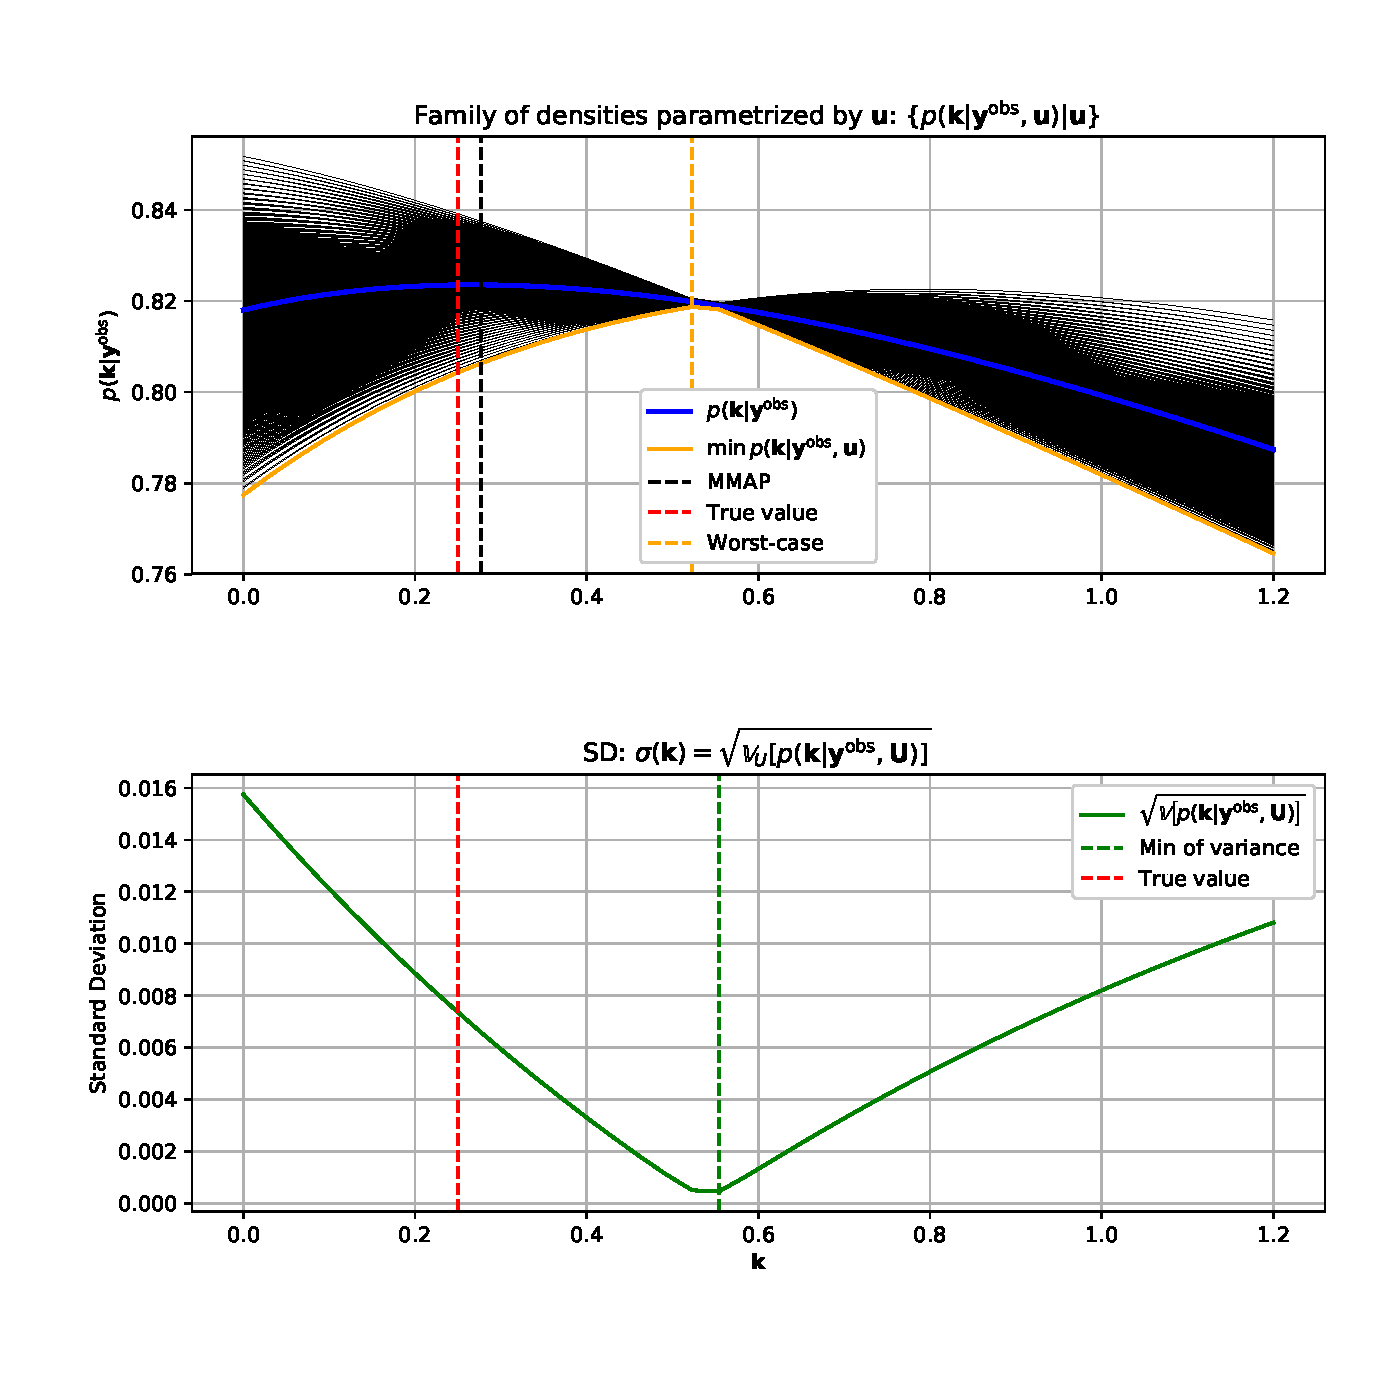
\includegraphics[width = \linewidth, height = .9\textheight]{MMAP_minvariance}
% \end{center}
% \end{column}
% \end{columns}
% }
% \frame{
%   \frametitle{``Most Probable Estimate''}
%   $\bm{K}_{\argmax}= \argmax_{\bm{k}\in\mathcal{K}} p(\bm{k} | \yobs,\alert{\bm{U}})$ random variable \\
%   $\longrightarrow$ estimate its density (how often is the value $\bm{k}$ a maximizer)

%   Straightforward algorithm:
%   \begin{itemize}
% \item For $i=1\dots N$:
%     \begin{itemize}
%   \item Sample $\bm{u}^{(i)}$ from $\pi(\bm{u})$ / Adapted space-filling designs
%   \item Maximize $p(\bm{k}|\yobs,\bm{u}^{(i)})$ yielding $\bm{k}_{\argmax}^{(i)}$ (adjoint method)
%   \end{itemize}
%   \item Estimate density (KDE) / Mode
%   \end{itemize}
%  }
% \frame{
%   \frametitle{Illustration of MPE}
                                %   \movie[width = \linewidth, height= \textheight, poster, showcontrols]{}{animation.mpg}
% }
% \section{Surrogates and optimization}
% \frame[t]{
% \frametitle{Why surrogates?}
% \begin{itemize}
% \item Computer model: \alert{expensive to run}
% \item $\dim \mathcal{K}$ , $\dim \mathcal{U}$ can be very large: \alert{curse of dimensionality}
% \item Uncertainties upon $\bm{u}$ directly in the surrogate
% \end{itemize}
% \vfill
% \begin{center}
% 	\only<1>{\scalebox{0.9}{\input{../Figures/comp_code_surro.pgf}}}	
% 	\only<2>{\scalebox{0.9}{
\tikzstyle{block} = [rectangle, draw, fill=blue!20, 
     text centered, minimum width=1cm]
\tikzstyle{block2} = [rectangle, draw, fill=green!20, 
     text centered, , minimum width=6cm]

\tikzstyle{LHS}=[rectangle, draw, text centered]

\begin{tikzpicture}[node distance=3cm]

\node [align = center] at (0,0) (input) {Control variable \\$K \in \mathcal{K}$};
\node [align = center] at (4,1.5) (envir) {Environmental variables \\$\bm{X}_e$ random};
\node[block] at (4,0)(code){Computer Code};
\node[align = center] at (7,0) (output) {$W(\bm{x}_e,K)$};
\node[align = center] at (9.2,0) (jfun) {$\bar{j}(\bm{x}_e,K)$};
\draw[->] (input) -- (code);
\draw[->] (envir) -- (code);
\draw[->] (code) -- (output);
\draw[->] (output) --(jfun);
\node[block2] at (5,0) (surr) {Metamodel};
\draw[->] (input) -- (surr);


\end{tikzpicture}}}
% \end{center}
% \vfill
% }
% \frame{
% \frametitle{Using surrogates for optimization : adaptative sampling}
% Based on kriging model ( =Gaussian Process Regression) $\longrightarrow$ mean and variance \\
% How to choose a new point to evaluate ? 
% Criterion $\kappa(\bm{x}) \longrightarrow$ "potential" of the point
% \begin{equation*}
% \bm{x}_{\mathrm{new}} = \argmax \kappa(\bm{x})
% \end{equation*}
% 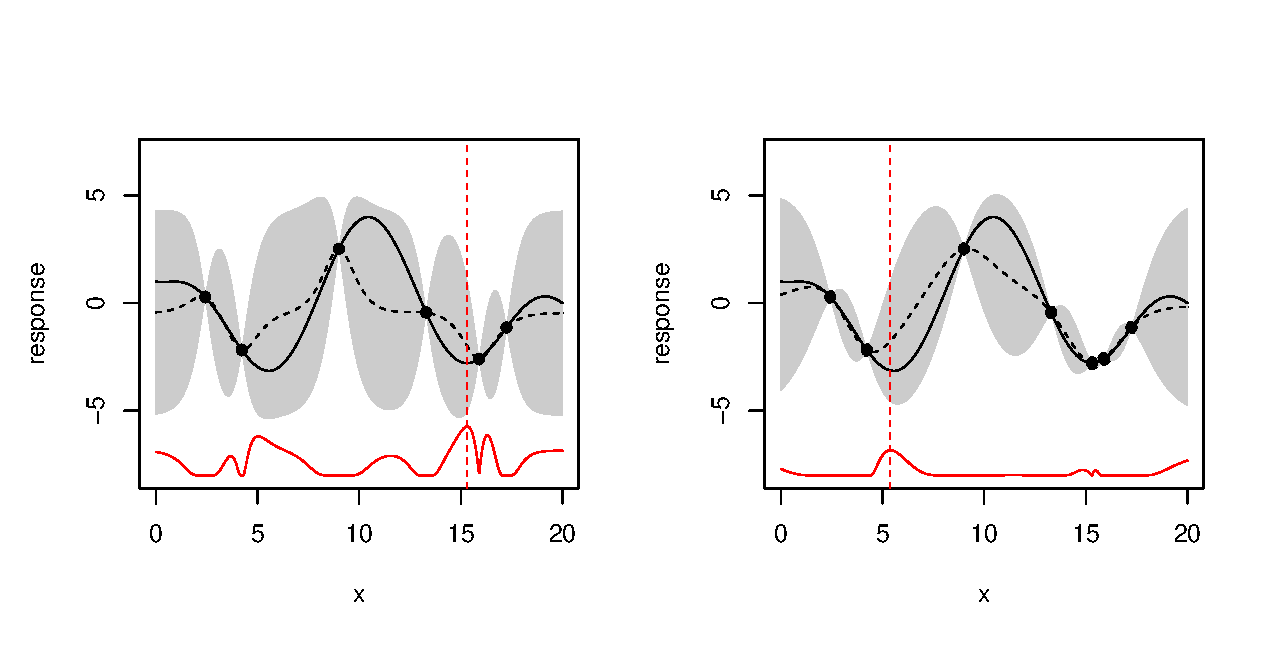
\includegraphics[width = \textwidth]{example_EGO}
% }

% \section{Conclusion}

\frame{
\frametitle{Conclusion}
\begin{block}{Interrogations}
\begin{itemize}
\item Fonction coût ou vraisemblance/postérieur ? ``Mêmes'' quantités, méthodes différentes pour les manipuler ?
\item Quels critères sont vraiment pertinents ? liens entre eux ?
\item À partir d'un ensemble de candidats: lequel choisir ?
% \item Modélisation de $\bm{U}$ ?
\item Quel budget d'évaluations en pratique ?
\end{itemize}
\end{block}


\begin{block}{À faire}
  \begin{itemize}
  \item Utilisation des métamodèles (sur quelles fonctions ?)    
  \item Ensembles aléatoires pour probabilité de défaillance (voir avec Reda)
  \item $\yobs$ ?
  \end{itemize}
\end{block}
}

\end{document}